\documentclass[12pt,spanish]{article}
\usepackage[utf8]{inputenc}
\usepackage[T1]{fontenc}
\usepackage{babel}
\usepackage{graphicx}
\usepackage{amsmath}
\usepackage{listings}
\usepackage{color}
\usepackage{hyperref}
\usepackage{geometry}
\geometry{margin=2.5cm}
\hypersetup{
    colorlinks=false,
    pdfborder={0 0 0}
}


\title{\textbf{Simulación Cooperativa del Juego de Caramelos-Superviviente}}
\author{Yonhel Mamani Cruz \\ Universidad Nacional del Altiplano de Puno}
\date{Julio 2025}

\begin{document}

\maketitle

\tableofcontents
\newpage

% ----------------------------------------
\section{Resumen}

Se presenta una simulación cooperativa del juego de caramelos y chupetines. El juego fue implementado en Python utilizando la biblioteca gráfica Tkinter. Cada jugador inicia con caramelos aleatorios, y el objetivo es conseguir al menos un chupetín por persona. Se implementó una lógica cooperativa para asegurar que todos los participantes logren el objetivo, incluso en casos donde existan grupos incompletos o jugadores individuales.

% ----------------------------------------
\section{Introducción}

El juego de caramelos y chupetines fue diseñado con el objetivo de fomentar el pensamiento lógico, la estrategia cooperativa y el trabajo en equipo. Esta dinámica lúdica ha sido transformada en un programa interactivo que simula el proceso de distribución y combinación de caramelos. El sistema promueve la colaboración entre jugadores, permitiendo asegurar que todos obtengan al menos un chupetín, incluso cuando la formación de grupos sea desigual.

% ----------------------------------------
\section{Descripción del Juego}

Cada jugador recibe inicialmente dos caramelos, seleccionados aleatoriamente entre los siguientes tipos:

\begin{itemize}
  \item Limón
  \item Huevo
  \item Pera
\end{itemize}

Para formar un chupetín, se requiere una combinación específica:

\begin{itemize}
  \item 2 caramelos de limón
  \item 2 caramelos de huevo
  \item 2 caramelos de pera
\end{itemize}

Una vez formado un chupetín, el jugador recibe dos caramelos adicionales. Existe también la posibilidad de vender un chupetín a cambio de seis caramelos nuevos, lo cual puede ayudar en momentos estratégicos del juego.

% ----------------------------------------
\section{Planteamiento del Problema}

Durante la ejecución del juego, surgen varios desafíos:

\begin{itemize}
  \item Asegurar que todos los jugadores obtengan al menos un chupetín.
  \item Manejo de grupos incompletos o jugadores individuales.
  \item Redistribución de caramelos para lograr combinaciones viables.
\end{itemize}

% ----------------------------------------
\section{Procedimientos y Desarrollo}

\subsection{Lógica de Grupos Incompletos}

En el juego pueden existir grupos que no tengan el número ideal de integrantes. Las estrategias aplicadas son:

\begin{enumerate}
  \item Los jugadores individuales pueden integrarse temporalmente a otros grupos.
  \item Los grupos incompletos pueden intercambiar caramelos con otros grupos.
  \item Se garantiza equidad mediante reglas cooperativas programadas.
\end{enumerate}

\subsection{Entradas del Usuario}

Al iniciar el programa, se solicitan dos datos fundamentales:

\begin{itemize}
  \item Número de jugadores
  \item Número de integrantes por grupo
\end{itemize}

\subsection{Fragmento de Código Utilizado}

\begin{lstlisting}[language=Python, caption={Validación para formar un chupetín}]
def can_make_chupetin(inv):
    return inv['limon'] >= 2 and \
           inv['huevo'] >= 2 and \
           inv['pera'] >= 2
\end{lstlisting}

% ----------------------------------------
\section{Resultados}

A continuación se presentan los resultados obtenidos durante una ejecución de prueba:

\begin{itemize}
  \item Se simularon 10 jugadores.
  \item Todos lograron formar al menos un chupetín.
  \item Se vendió un chupetín para obtener caramelos adicionales.
  \item Un grupo fue formado por un solo jugador, quien se integró temporalmente a otro grupo.
\end{itemize}

% ----------------------------------------
\section{Evidencias del Procedimiento}

A continuación, se incluyen capturas de pantalla como evidencia del desarrollo y ejecución del programa:

\begin{figure}[h!]
  \centering
  
\includegraphics[width=0.9\textwidth]{cara1.png}
  \caption{Inicio de la simulación - ingreso de datos}
\end{figure}

\begin{figure}[h!]
  \centering
  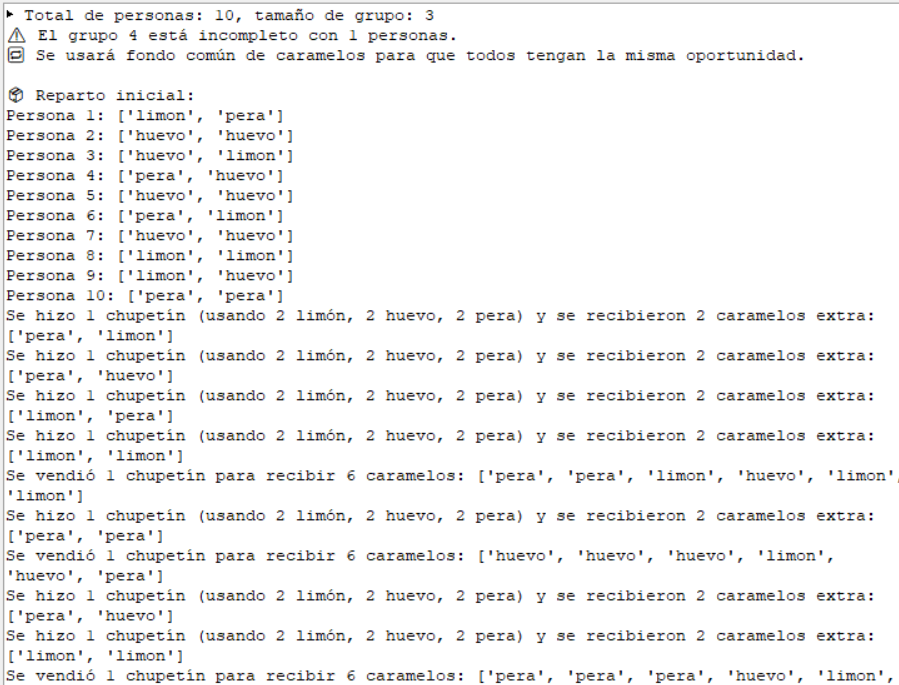
\includegraphics[width=0.9\textwidth]{cara2.png}
  \caption{Visualización de caramelos iniciales por jugador}
\end{figure}

\begin{figure}[h!]
  \centering
  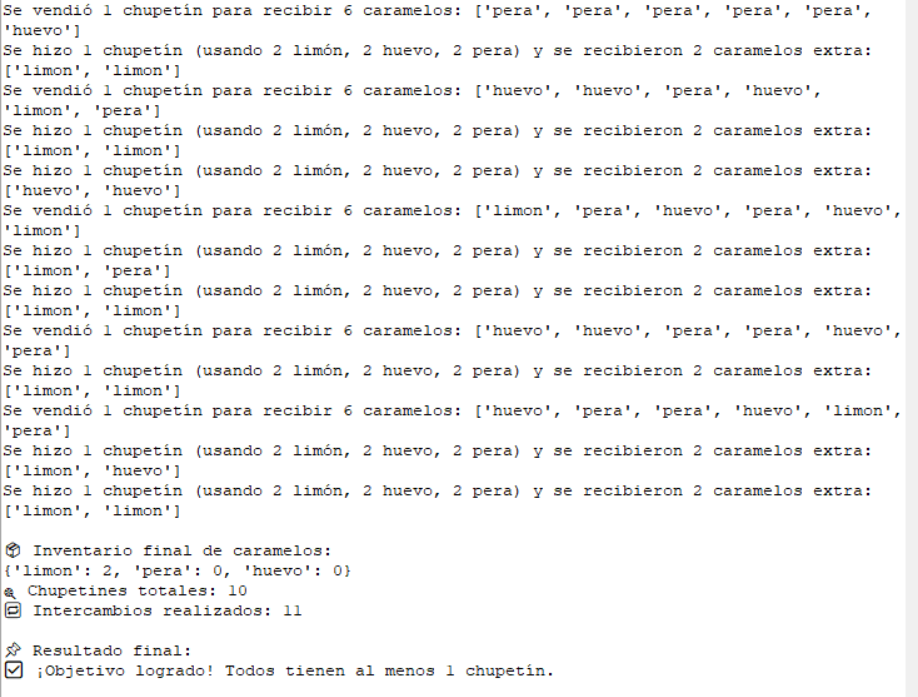
\includegraphics[width=0.9\textwidth]{cara3.png}
  \caption{Proceso de combinación y creación de chupetines}
\end{figure}

\begin{figure}[h!]
  \centering
  
\includegraphics[width=0.9\textwidth]{cara4.png}
  \caption{Resultado final con todos los jugadores ganando}
\end{figure}

\clearpage

% ----------------------------------------
\section{Conclusiones}

La simulación desarrollada del juego de caramelos y chupetines permitió abordar un problema de asignación y cooperación desde una perspectiva de optimización discreta. Se implementaron estrategias que buscan maximizar la obtención de chupetines por parte de los jugadores, bajo restricciones de recursos limitados (caramelos) y combinaciones específicas.

La lógica del sistema garantizó soluciones factibles incluso en escenarios con grupos incompletos o jugadores individuales, demostrando la eficiencia del algoritmo en la redistribución equitativa de recursos. Asimismo, se logró minimizar el desperdicio de caramelos mediante intercambios y decisiones cooperativas, lo cual refleja una optimización del uso de insumos.

En conjunto, el simulador constituye una aproximación lúdica a problemas clásicos de optimización combinatoria y asignación de recursos, con aplicaciones potenciales en el análisis de estrategias colaborativas, juegos serios y educación computacional.


% ----------------------------------------
\end{document}


